%\documentclass[a4j,12pt,twocolumn]{jsik}
\documentclass[12pt,a4paper,twocolumn,twoside]{jsik}
\usepackage{balance}
\usepackage{float}

\begin{document}

\pagestyle{empty}
\thispagestyle{empty}

\articletype{第34回年次大会予稿}
\jtitle{地域研究活動の指標開発にむけて \\ - 文書からの地名抽出 -}
\etitle{Towards the development of indicators for regional studies \\ - Extraction of place names from documents -}
\jauthor{黄秋実$^{1}$, 寺田将春$^{1}$, 上村麻里亜$^{1}$, 船守美穂$^{1,2}$, 天野晃$^{1*}$}
\eauthor{Qiushi HUANG$^{1}$, Masaharu TERADA$^{1}$, Maria KAMIMURA$^{1}$, Miho FUNAMORI$^{1,2}$, Kou AMANO$^{1*}$}
\affiliation{
  \begin{tabbing}
1 鹿児島大学 \\
\ 〒890-8580 鹿児島県鹿児島市郡元1丁目21-24 \\
2 国立情報学研究所 \\
\ 〒101-8430 東京都千代田区一ツ橋2-1-2 \\
\ E-mail: k7085637@kadai.jp \\
$*$ 連絡先著者
  \end{tabbing}
}

\jabstract{
近年我が国では、多くの地域において少子高齢化や人口流出により労働人口が減少し、地域課題の解決が困難になりつつある。これに対し、文部科学省は地方大学にその解決への取り組みを期待している面がある。実際、多くの大学も自身の存在意義を示すために地域に根ざした研究に力を入れている。一方で、計量書誌学の観点からは、このような地域研究の活動を示すような指標の開発はあまり見られない。これにはいくつかの問題があるからだと考えられる。まず、地域の名称（地名）を文章等から正しく抽出することが困難であり、つぎにその地名が唯一に決められるかも難しい問題である。最終的には対象となる論文やデータに対して地名や地理情報をユニークに紐づける（キュレーションする）仕組みが必要となる。本研究では、このようなソリューションを視野に入れるものの、まずは地名の抽出という問題に着目し、コンパクトなテストデータを用いた試みを行う。
}

\eabstract{
In recent years in Japan, the working-age population has been declining in many regions due to a falling birthrate, an aging population, and outmigration, making it increasingly difficult to address regional challenges. In response, the Ministry of Education, Culture, Sports, Science and Technology (MEXT) has, in part, placed expectations on regional universities to contribute to solving these issues. In fact, many universities are strengthening research rooted in their local communities in order to demonstrate their own significance.
On the other hand, from a bibliometric perspective, there has been little development of indicators that capture such region-oriented research activities. This is likely due to several challenges. First, it is difficult to accurately extract place names (toponyms) from texts and other materials. Second, it is also challenging to uniquely identify and disambiguate those place names. Ultimately, there will be a need for mechanisms to uniquely link place names and geographic information to the relevant papers and datasets.
While this study takes such solutions into consideration, it first focuses on the accuracy of place name extraction and conducts an experimental study using a compact test dataset.
}


\keywords{
固有表現抽出 (NER), 形態素解析, 地域課題, AI\\
Named Entity Recognition (NER), Morphological analysis, regional issues, AI
}

\maketitle

　　　 \\
　　　 \\
　　　 \\

\begin{figure*}[h]
\begin{center}
  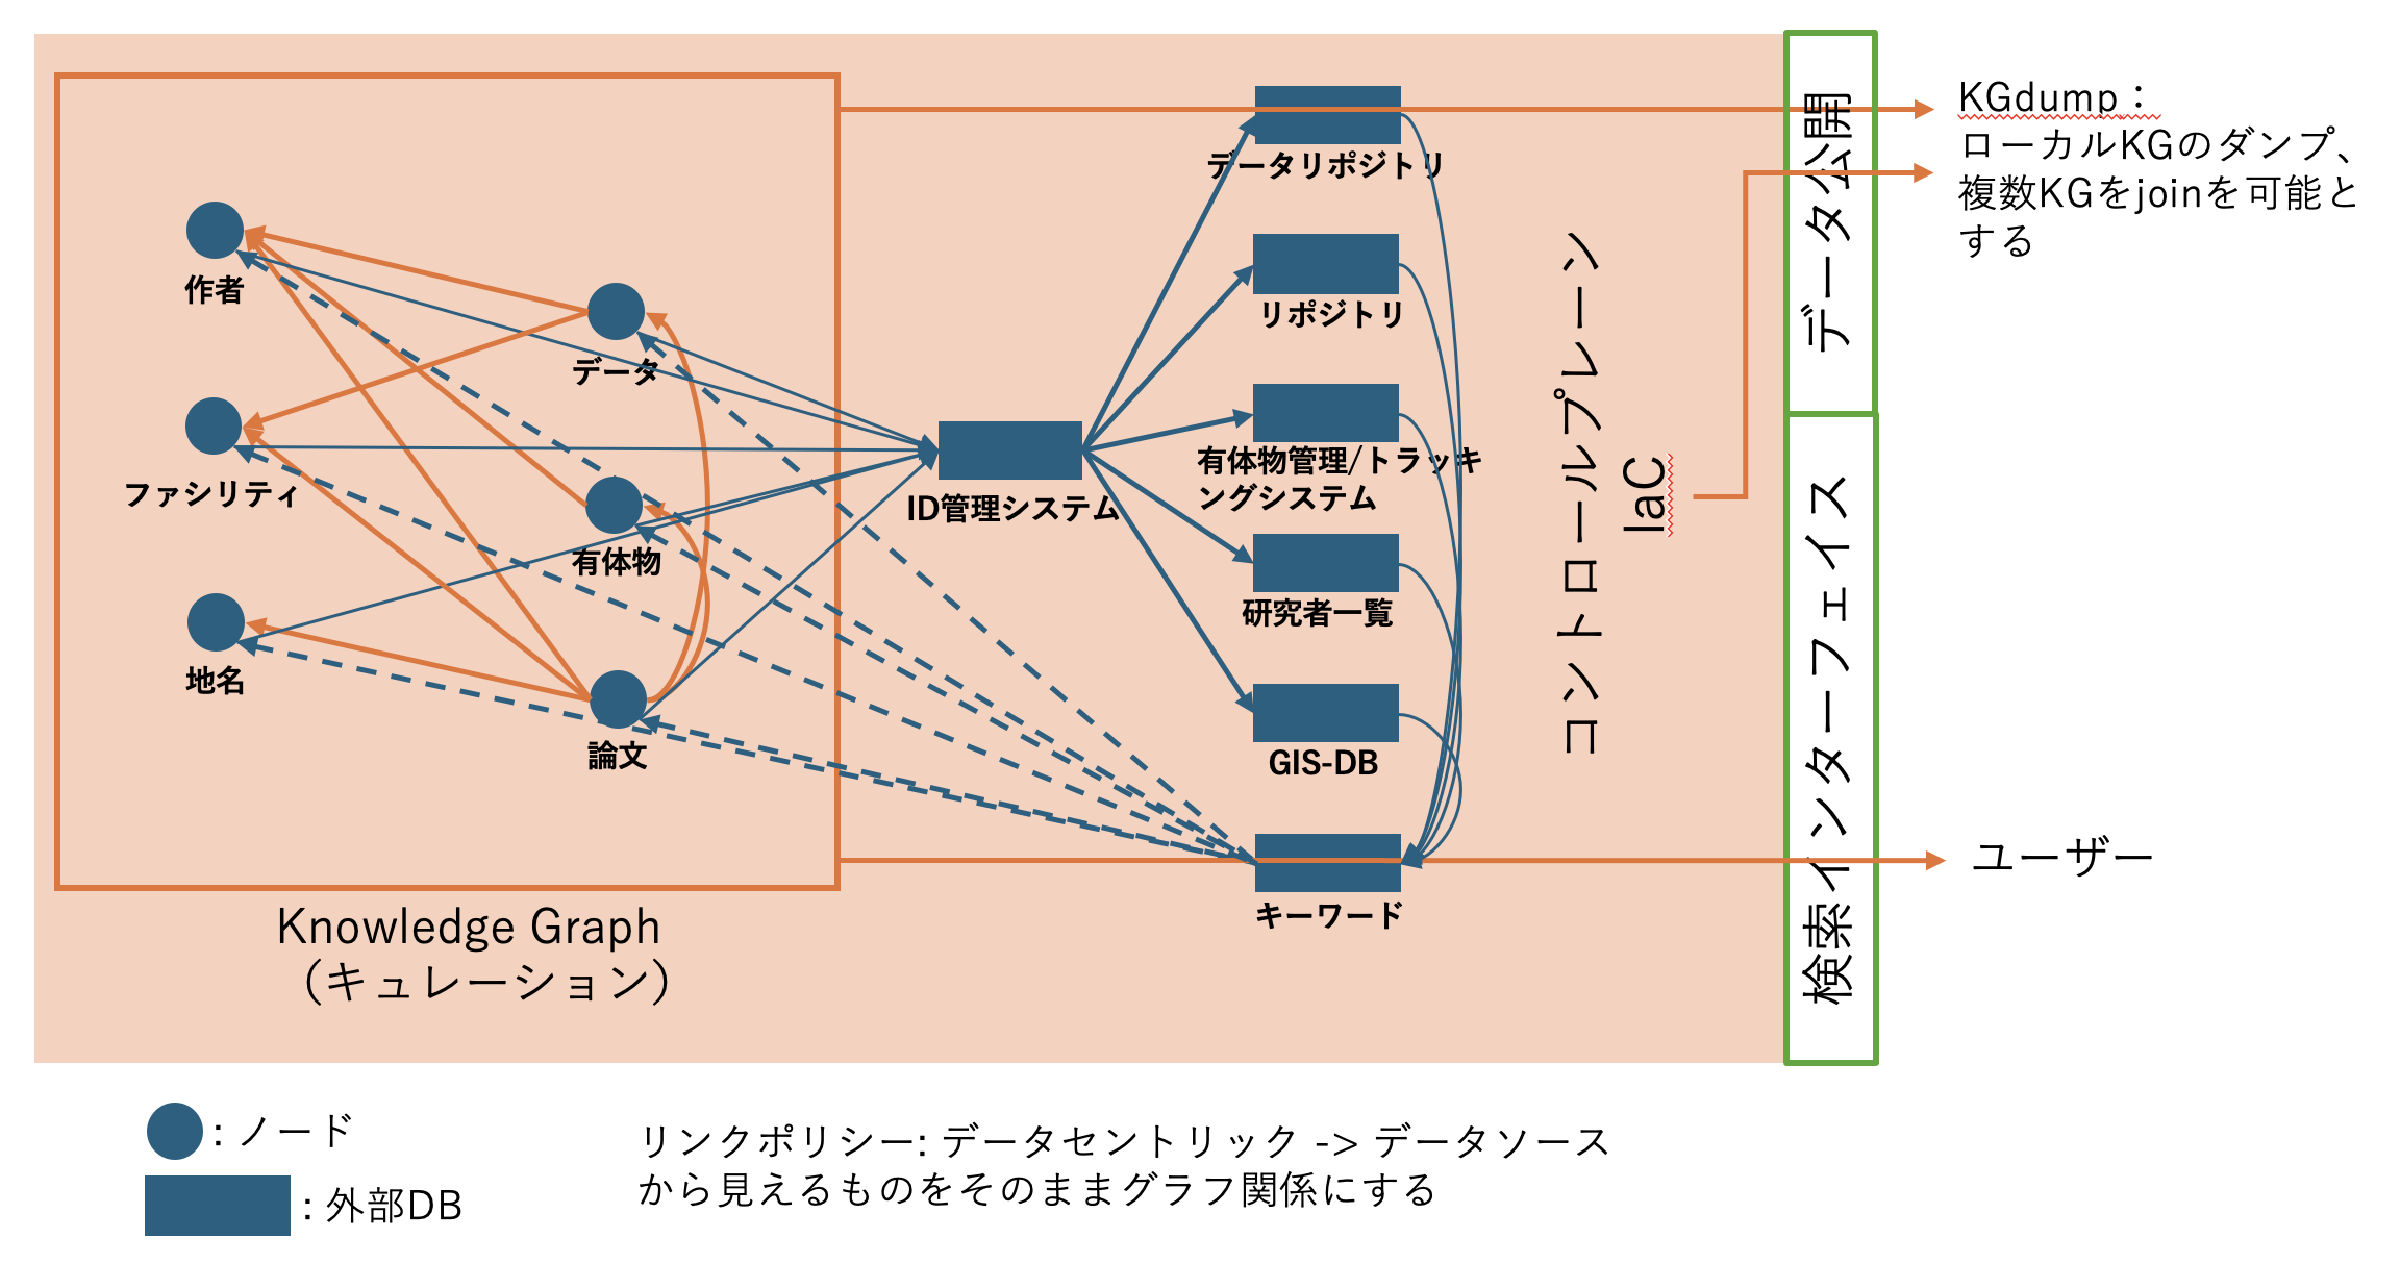
\includegraphics[width=160mm]{kgview.eps}
  \caption{固有表現抽出による知識グラフ}
  \label{fig:kg}
\end{center}
\end{figure*}

\section{背景}
本学では、2025年4月にオープンサイエンス研究開発部門が附属図書館の下部組織として発足した\cite{kgos1}。当部門は、学内外の組織との協力・協調のもとに地域課題解決を目指す「KAGOSHIMAモデル」\cite{kglib1}を推進するための中心的な部局である。
地方大学である本学では、地域社会への貢献が重要な任務であると同時に、その成果をどのように発信あるいは見える化するかもまた、重要な課題となっている。このような会活動・社会貢献にかかる指標開発や分析は、活動そのものを把握し、より効果的に推進するために必要なものとなる。

本部門ではこのための試験的な活動の一環として、ドキュメントから固有表現を抽出しその関係性を整理する仕組みの開発を構想しており（図\ref{fig:kg}）、その第一段階としてAIを導入した地域（地名）を対象とした固有表現抽出（NER）の試みとその評価を行った。


\section{目的}
地域研究活動の指標開発の一環として、文章からの正しい地域名（人名等を含まない）の抽出を目指す。その方法の一つ、地域名称を形態素解析により抽出しさらにAIに判定させる方法を試行し、評価する。


\section{マテリアル・方法}
まず，KAKENデータベース\cite{kaken1}より，国立大学による報告書を収集した．本研究ではこのうちランダムに選択した4大学の報告書からさらにランダムに各大学につき50件を抽出し，対象とした．地名の抽出対象は研究課題名および報告書本文とした．
次にmecab\cite{mecab}により固有表現抽出（形態素解析）を行い，"固有名詞"および"地域"のラベルがあるものを抽出した．これらに対し，さらにmecabの判定が妥当かを複数の判定者に判定させた．判定者は3種のAIと3名の人とした．
判定者へは，AI，人ともに表\ref{tab:prompt}（視認性のため文には改行・空白を挿入している）の指示を与えた．データは4要素からなるJSON形式で与え，第2要素を抽出された地名，第4要素を研究課題名および本文（すなわち固有表現抽出の対象）とした．それ以外の要素は管理目的で挿入したものであり無視するよう促した．なお，AIには，Gemma3（4b）\cite{gemma3}，Llama3（8b）\cite{llama3}，Qwen3（32b）\cite{qwen3}を用いた．期待する出力形式は，入力されたJSONの第2要素に対する修正がなされたJSONである．AIの判定実行はローカルAI環境（Ollama\cite{ollama}）により1報告書ごとに行った．判定はAIに関しては一回のみ実行し，人に対しては期限を設け，複数回の提出を認めた．
最後に，判定結果を集計し，分析した．

\begin{table*}[h]
\begin{center}
\caption{プロンプト} \label{tab:prompt}
\begin{tabular}{lp{86mm}}
\multicolumn{2}{l}{添付のデータに対して以下の作業を行って下さい。} \\
- 概要 : & 地名候補を地名であるか判定する。 \\
- 入力データ形式 : & json形式、4 つの要素から成る。各要素はさらに配列である可能性がある。 \\
- 入力データの各要素の説明 : & {}  \\
\ - 第1要素 : & 無視して良い \\
\ - 第2要素 : & 第4要素から抽出された地名候補 \\
\ - 第3要素 : & 無視して良い \\
\ - 第4要素 : & 文章（配列） \\
- 行ってほしい作業 : & jsonの第2要素の各地名候補が地名であるかを、第4要素の文脈から判定してほしい。 \\
- 出力データ形式 （判定結果） : & 第2要素のみを次のように出力する : 第2要素の地名候補が地名であればそのまま残し、そうでない場合は0に置きかえたもの。 \\
\end{tabular}
\end{center}
\end{table*}


\section{結果}
\subsection{出力形式の評価}
各判定者の出力に対し、求められた正しい形式（JSON）になっているかを評価した。人による判定結果は全てがワンライナーのJSON形式であった。AIによる判定結果の多くは判定理由とともにコードブロックもしくはワンライナーの形式で判定結果を出力していたため、まず、コードブロックもしくはJSONのワンライナー部分をを抽出した。ただし、AIのうち一つはほとんどの出力形式が不適合であったためこの段階で本研究の対象外とした。表\ref{tab:hanteiform}に各判定者がJSON形式を正しく出力した数を示す。

\begin{table}[h]
\begin{center}
\caption{判定の出力形式} \label{tab:hanteiform}
\begin{tabular}{lc}
判定者 & 正しいJSON形式 \\
AI 1 & 141 / 200 \\
AI 2 & 対象外 \\
AI 3 & 149 / 200 \\
Human 1 & 200 / 200 \\
Human 2 & 200 / 200  \\
Human 2 & 195 / 200  \\
\end{tabular}
\end{center}
\end{table}


\subsection{判定結果の評価}
\subsubsection{判定者の分類}
mecabによる地名の抽出結果および各判定者により修正されたデータ間のクラス構造を確認するため，6データ全てに対し，415箇所の判定箇所を対象としたハミング距離を用いたクラスタリングを行った．この結果を図\ref{fig:dg}に示す．概ね人とAIに分かれ，AIは修正の度合いが小さい（元データに近い）ように見受けられる．改めてこの距離行列を表\ref{tab:diff}に示す．人の判定においても相当の差異が生じており，地名判定の難しさを物語っている．

\begin{figure}[h]
\begin{center}
  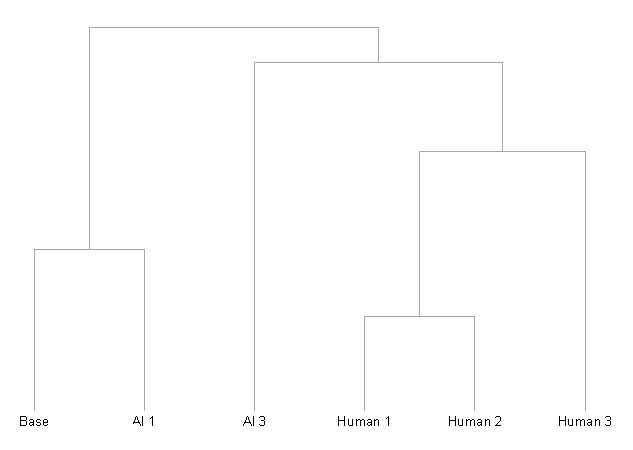
\includegraphics[width=76mm]{dg.eps}
  \caption{AI・人による判定の差のデンドログラム}
  \label{fig:dg}
\end{center}
\end{figure}

\begin{table*}[h]
\begin{center}
\caption{判定者間のハミング距離} \label{tab:diff}
\begin{tabular}{cccccc}
 {Base} & {AI 1} & {Human 1} & {Human 2} & {Human 3} & {AI 3} \\
\hline
 0 & 51 & 127 & 127 & 141 & 121 \\
 51 & 0 & 142 & 136 & 156 & 137 \\
 127 & 142 & 0 & 30 & 84 & 123 \\
 127 & 136 & 30 & 0 & 82 & 110 \\
 141 & 156 & 84 & 82 & 0 & 120 \\
 121 & 137 & 123 & 110 & 120 & 0 \\
\end{tabular}
\end{center}
\end{table*}


\begin{table*}[h]
\begin{center}
\caption{判定者による修正数} \label{tab:countrev}
\begin{tabular}{cccccc}
 {Base} & {AI 1} & {Human 1} & {Human 2} & {Human 3} & {AI 3} \\
\hline
 0 & 28 & 127 & 127 & 141 & 95 \\
\end{tabular}
\end{center}
\end{table*}

\subsubsection{判定者による修正の程度}
判定による修正数を表\ref{tab:countrev}に示す。
次に、大学間で判定に差異があるかを確認する。まず表\ref{tab:report}に大学ごとのドキュメント数を示す。ドキュメントの修正の程度のヒストグラムを図2に示す。ヒストグラムの形状はいずれも同じ傾向に見えるが、さらにKruskal-Wallis法\cite{krunkallwallis}による検定を行った結果、P値は0.029であり有意差があると考えた方が良い。

\begin{table}[H]
\begin{center}
\caption{各大学の報告書数} \label{tab:report}
\begin{tabular}{lc}
大学 & 報告書数 \\
\hline
大学 1 & 26 \\
大学 2 & 17 \\
大学 3 & 31 \\
大学 4 & 25 \\
\end{tabular}
\end{center}
\end{table}

\begin{figure*}[h]
\begin{center}
  {\small
  \begin{tabular}{cc}
  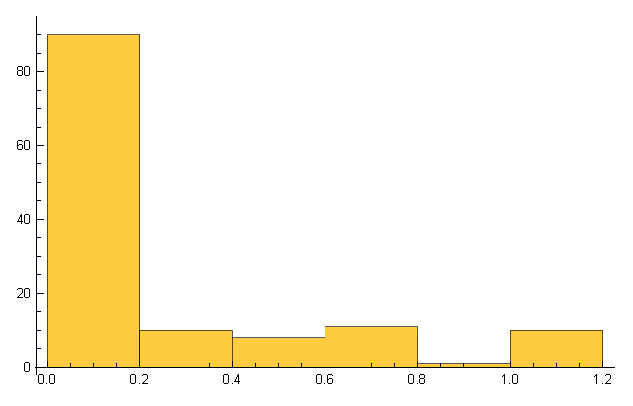
\includegraphics[width=75mm]{hst1.eps} & 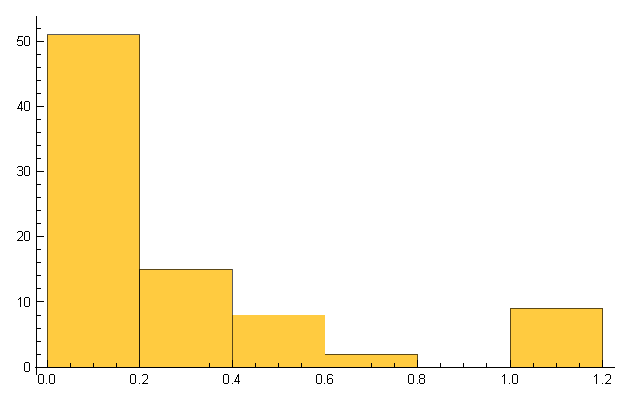
\includegraphics[width=75mm]{hst2.eps} \\
  大学 1 & 大学 2 \\
  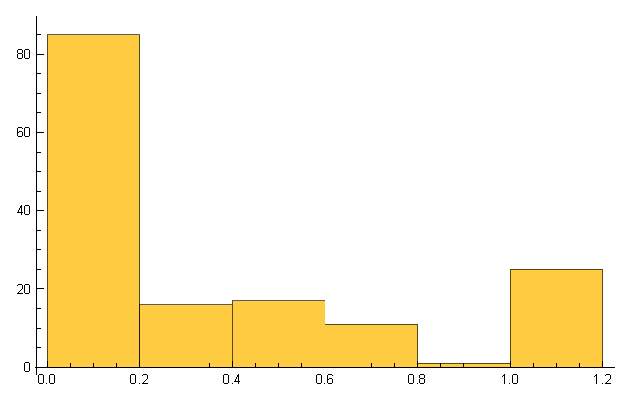
\includegraphics[width=75mm]{hst3.eps} & 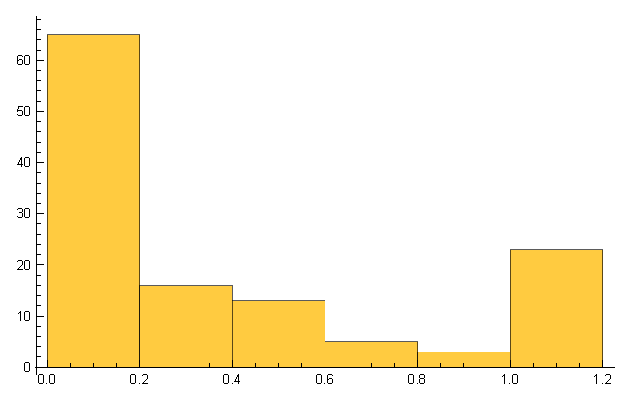
\includegraphics[width=75mm]{hst4.eps} \\
  大学 3 & 大学 4 \\
  \end{tabular}
  }
  \caption{修正の程度のヒストグラム}
  \label{fig:hst}
\end{center}
\end{figure*}


\balance
\subsubsection{地名の決定について}
\textbf{地名の決定}

AIおよび人による各判定から，地名であるかを決定するため多数決によ決定を行った．この結果，mecabにより地名とされた141タームのうち，99タームが地名と判定された．一方，地名でないと判断されたタームは45ターム，地名であると判定された場合も地名でないと判定された場合もあるタームは3タームであった．なお，以上の数値はいずれもユニーク数である．


\textbf{決定された地名の例}

抽出・決定された地名の中には1文字の「仏」，「米」等の国名の略記がそれなりに見られた．これらはおもに複数国を示す複合要素として出現していたが，ほとんどの場合正しく抽出・判定されていた．一方，同様に国名の略記であるにもかかわらず「日」，「中」など一部のものについては，固有表現抽出では地名として抽出されているにもかかわらず，判定では地名と見なされない場合が多かった．その他興味深いものとして，「集」のようなあまり馴染みのない地名を正しく実在する地名として抽出した例があった．


\textbf{大学ごとの地名出現の差異}

次に，大学ごとに地名の出現に差があるかを，各大学間（ペアワイズ）のDice係数で確認した（表\ref{tab:dice}）．係数の値は0.07から0.29と幅があるがいずれも低い傾向にあり，大学ごとに嗜好があることが示唆される．

\begin{equation}
\frac{2 |A \cap B|}{|A|+|B|}
\label{eq:dice}
\end{equation}

\begin{table}[h]
\begin{center}
\caption{大学間の地名出現のDice係数} \label{tab:dice}
\begin{tabular}{cccc}
大学 1 & 大学 2 & 大学 3 & 大学 4 \\
\hline
 1.& 0.07& 0.07& 0.14 \\
 0.07& 1.& 0.12& 0.21 \\
 0.07& 0.12& 1.& 0.29 \\
 0.14& 0.21& 0.29& 1. \\
\end{tabular}
\end{center}
\end{table}


\section{まとめ・今後の課題}
固有名称抽出（形態素解析）による地名の判定と、AI・人による地名の判定には大きな隔たりがあり、今回の研究では最小でも7\%（AI）、最大で34\%（人）が異なるはんていであった（表\ref{tab:countrev}より）。


\section{データ利用可能性宣言}
本研究で作成した，あるいは分析に用いたデータセットは（リポジトリ名称）の（DOI等の永続的識別子またはURL）で入手可能である．



%\footnote{http://masao.jpn.org/software/jsik\_bst/} が同封されています．

\balance
\bibliographystyle{jsik}
\bibliography{takaku}
%\begin{thebibliography}{0}
%\bibitem{aaa} あいうえお
%\end{thebibliography}
%\begin{thebibliography}{1}
%\bibitem{ex1}
% 藤原譲: 「情報知識学試論」, 情報知識学会誌, Vol.~1, No.~1, pp. 3--10, 1990.
%\bibitem{ex2}
% 原正一郎; 安永尚志: 「国文学研究支援のためのSGML/XMLデータシステム」,
%  情報知識学会誌, Vol.~11, No.~4, pp. 17--35, 2002.
%\end{thebibliography}

\end{document}
